%!TEX root = ../../master.tex
\chapter{Experiment: Evaluating Application Level and Infrastructure Level Resilience}
\label{chapter_experiment2_resilience}

\begin{theorem}
KubeCloud allows for physical experimentation that cannot be done using cloud providers.
Experimenting with resilience at the infrastructure and application level is a key feature in order to demonstrate the new paradigm of embracing failure.
\end{theorem}

\noindent
Until now, we have covered many different topics. In the introduction, we described the paradigm shift from monolithic applications to distributed microservice architectures and the increased complexity this architectural style brings. This increased complexity requires new methods to ensure resilience, and thereby new ways of teaching are needed. As described in Chapter~\ref{chap_fundamentals_resilient_cloud}, we outline methods to achieve resilience as application level and infrastructure level. Nygard describes multiple patterns for achieving a higher degree of resilience in production systems. However, to our knowledge, proper experiments have not been performed to verify the effects of these patterns. KubeCloud provides a controlled test environment in which it is possible to conduct experiments with these patterns e.g. pulling a network cable in a cloud provider's data center is not possible. Furthermore, these experiments will underpin the importance of designing for failure and support the students' understanding of resilience. The students have further conducted the following experiments to verify the results: application level resilience and infrastructure level resilience regarding recovery time. \\

\noindent
All tests in this section are performed using a load testing tool, Vegeta.


%%% Experiment 1.1
\section{Application Level Experiments}\label{sec:exp_integration_points}
\subsection*{Design of Experiment: Integration Points in a Synchronous Architecture}
Application level resilience refers to methods that can be applied by the developer to achieve a higher degree of resilience. The experiments described in this section will focus on integration points in a synchronous architecture and the derived antipatterns. We will investigate the effects of applying patterns as a solution to these antipatterns. \\

\noindent
Integration points in a synchronous architecture must be handled with care. Nygard describes integration points as \textit{"[...] the number-one killer of systems"} \cite[p. 46]{nygard2007release}. He points out that timeouts and circuit breakers can be a solution. This experiment illustrates and documents the effects of circuit breakers when a service becomes unresponsive. \\

\noindent 
The test setup consists of three services running in KubeCloud. The three services form a chain in which Service 0 requests resources from Service 1 through HTTP, and Service 1 requests resources from Service 2 also through HTTP. A delay of 15 seconds is introduced in Service 2 to simulate an unresponsive and strained service. The services are implemented in Spring Boot using Netflix's circuit breaker (Hystrix). Further details and implementation examples can be found in Appendix~\ref{appendix:application_layer}. This experiment will investigate three scenarios with a varying amount of circuit breakers. The scenarios are the following: \\

\noindent
\textit{1: No circuit breakers}
\\
In the first scenario, all requests between services are synchronous calls without timeouts or circuit breakers (Figure~\ref{fig:exp2_no_circuit_breaker}). The expected result is requests piling up between Service 1 and Service 2 because of slow responses leading to blocked threads. The blocked threads should lead to a cascading failure making Service 1 unavailable and, at some point, Service 0 unavailable.

\begin{figure}[H]
\centering
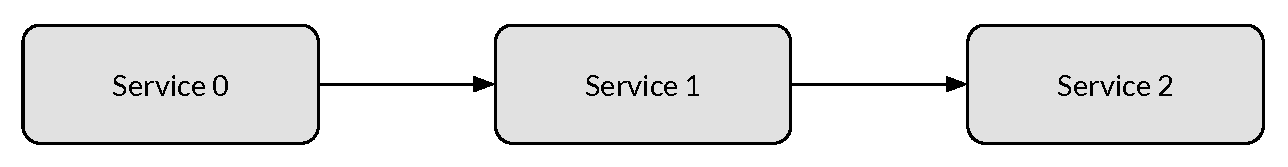
\includegraphics[scale=0.5]{figures/no_circuit_breaker_3_services}
\caption{Services without Circuit Breakers}
\label{fig:exp2_no_circuit_breaker}
\end{figure}

\noindent
\textit{2: One circuit breaker}
\\
In the second scenario, a timeout at 1 second between Service 1 and Service 2 is added. Furthermore, a circuit breaker is placed between Service 1 and Service 2 (Figure~\ref{fig:exp2_one_circuit_breaker}). The expected result is an improved overall response time since Service 1's timeout decreases time spent in blocked threads. Furthermore, the circuit breaker shuts off Service 2 at some point because of its slow responses.

\begin{figure}[H]
\centering
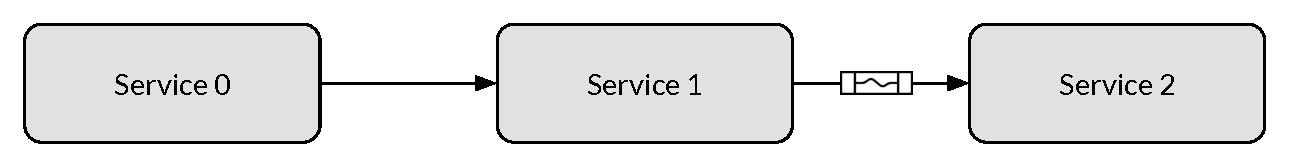
\includegraphics[scale=0.5]{figures/one_circuit_breaker_3_services}
\caption{Services with One Circuit Breaker}
\label{fig:exp2_one_circuit_breaker}
\end{figure}

\noindent
\textit{3: Two circuit breakers}
\\
In the third scenario, a timeout at 1 second between Service 0 and Service 1 together with a timeout at 1 second between Service 1 and Service 2 is added. Furthermore, a circuit breaker is placed between Service 0 and Service 1 together with a circuit breaker between Service 1 and Service 2 (Figure~\ref{fig:exp2_circuit_breaker}). The expected result is lower latencies since the timeout between Service 0 and Service 1 is reduced to 1 second.

\begin{figure}[H]
\centering
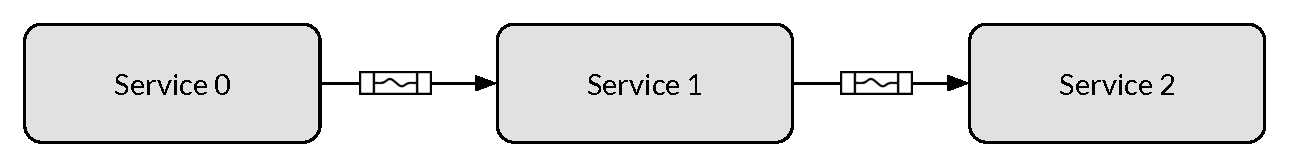
\includegraphics[scale=0.5]{figures/circuit_breaker_3_services}
\caption{Services with Two Circuit Breakers}
\label{fig:exp2_circuit_breaker}
\end{figure}


\noindent The expected result is that more circuit breakers lead to lower latencies and a higher success rate for requests. The results are expected to be degraded responses in the form of more fallback answers from Service 0 and Service 1. \\

\noindent Without circuit breakers, the requests are expected to block all threads because of Service 2's delay leading to blocked threads in the rest of the services while more requests are piling up. \\

\noindent 
When applying a circuit breaker between Service 1 and Service 2, the latencies are expected to be lower than the scenario without circuit breakers because Service 1 fails fast - the timeout is set to 1 second. \\

\noindent 
With two circuit breakers, the lowest latency is expected since the test runner's requests are directed towards Service 0 that has timeout is set to 1 second. If the circuit breaker can keep up with the request rate, the latency should not exceed much more than 1 second. Another interesting aspect is the amount of fallback responses from Service 0 and Service 1. \\

\noindent
\textbf{Test Protocol}
\\
For each iteration in each scenario, the same state must be created. In order to do so, a single instance of each service is started. In Kubernetes, this is achieved with a deployment with a single pod and an exposed service in front. When all three services are ready, two requests to Service 0 are made with 10 seconds delay. This ensures all services are ready, and that the circuit breakers, if present, are in the \textit{closed} state. \\
After 15 seconds, which is the duration of the delay in Service 2, the test runner can be started. The test runner generates 100 requests/second for 30 seconds which leads to 3000 measurements.\\

\noindent
When the test runner has finished, the Kubernetes pods are deleted and fresh instances created. The test protocol steps can then be repeated. Tests are executed from a MacBook Pro running an HTTP load testing tool called Vegeta which makes requests to Service 0 through a cabled network. \\

\noindent
\textbf{Metrics} \\
The main metrics from the experiments are \textit{latency}, \textit{success rate} and \textit{level of degradation}.\\

\noindent
The latency is a value between 0s and 30s since the test runner's timeout is set to 30s. The success rate is based on the HTTP status codes returned. 200 denotes a success, and 206 denotes a success from a circuit breaker. The level of degradation is measured as the distribution of the responses' origins. Response from Service 2 is the desired and best response. Subsequently, Service 1 is preferred over Service 0. \\


\noindent
\textbf{Data Basis}
\\
Three iterations of each scenario are run to reduce the impact of random factors. In each iteration, 3000 measurements will be made which sums up to 9000 measurements per scenario.

\subsection*{Results of Experiment: Integration Points in a Synchronous Architecture}
The results of the experiment show that circuit breakers lead to lower latencies, fewer timeouts and a different distribution of the responses' origins. \\

\noindent
\textbf{Latency} \\
 The histograms (Figure \ref{fig:circuit_breakers}) show normalized distributions of the response times for each scenario and a combination (a). \\
 
\noindent
Without circuit breakers (b), more than 9 of 10 latency measurements are measured as a value around 30 seconds, which is the test runner's timeout. The small section between 15 and 20 seconds are successful responses. These responses are in all three iterations around the first 200 responses after which the occurrences drastically decrease. The high amount of timeouts is most likely caused by blocked threads in Service 2 leading to a cascading failure. \\
 
 \noindent
Adding a circuit breaker in Service 1 (c) leads to lower response times, though, still several seconds. This is expected because of the reduced time spent in blocked threads in Service 1. The reduced time is caused by the timeout and a state change in the circuit breaker from \textit{closed} to \textit{open} state. No timeouts in the test runner were triggered after the addition of a circuit breaker.\\
 
\noindent The last scenario with two circuit breakers (d) led to drastically reduced response times. As expected, these values were mostly lower than the timeout of Service 0 which is 1 second. It makes sense that moving the circuit breaker closer to the caller reduces the latency since the undesired external factors are shielded by the circuit breaker.
 

\begin{figure}[H]%
    \centering
    \subfloat[Combined]{{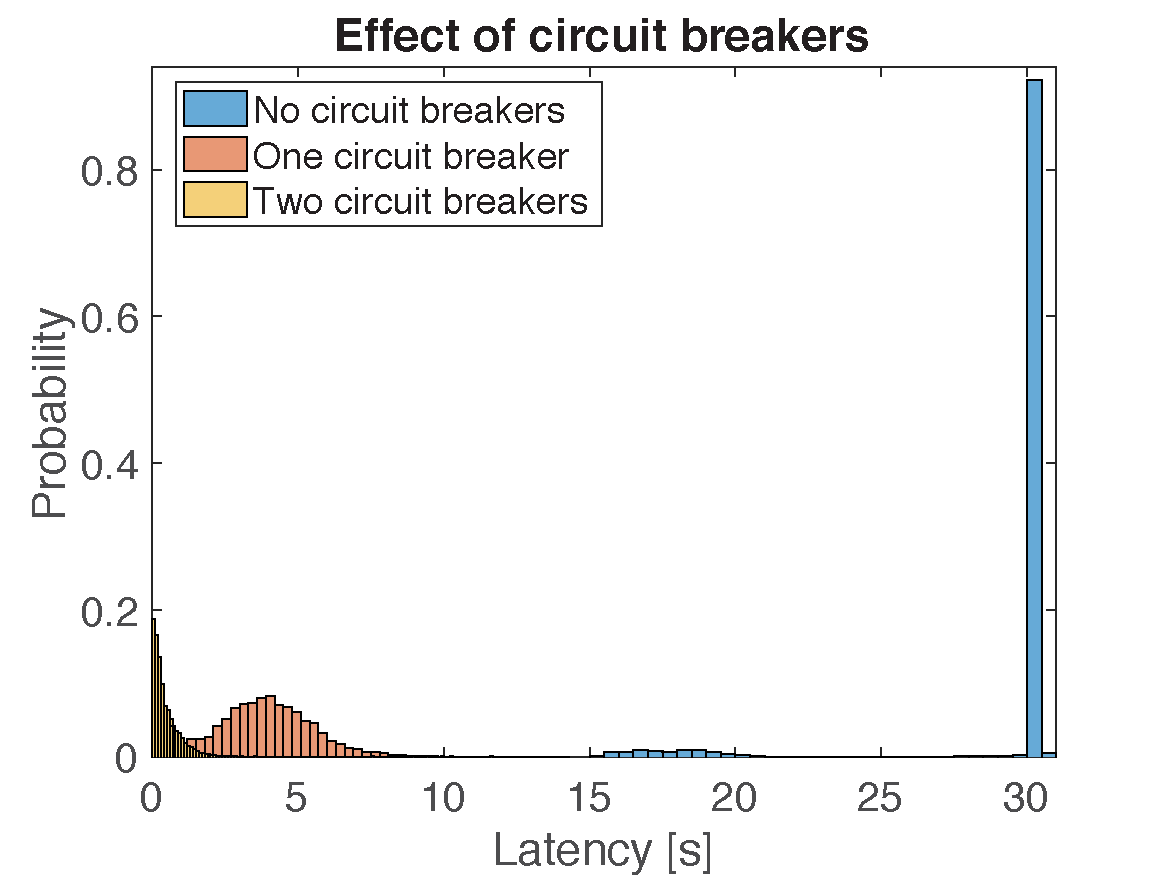
\includegraphics[width=7cm]{figures/all} }}%
      \qquad
    \subfloat[No circuit breakers]{{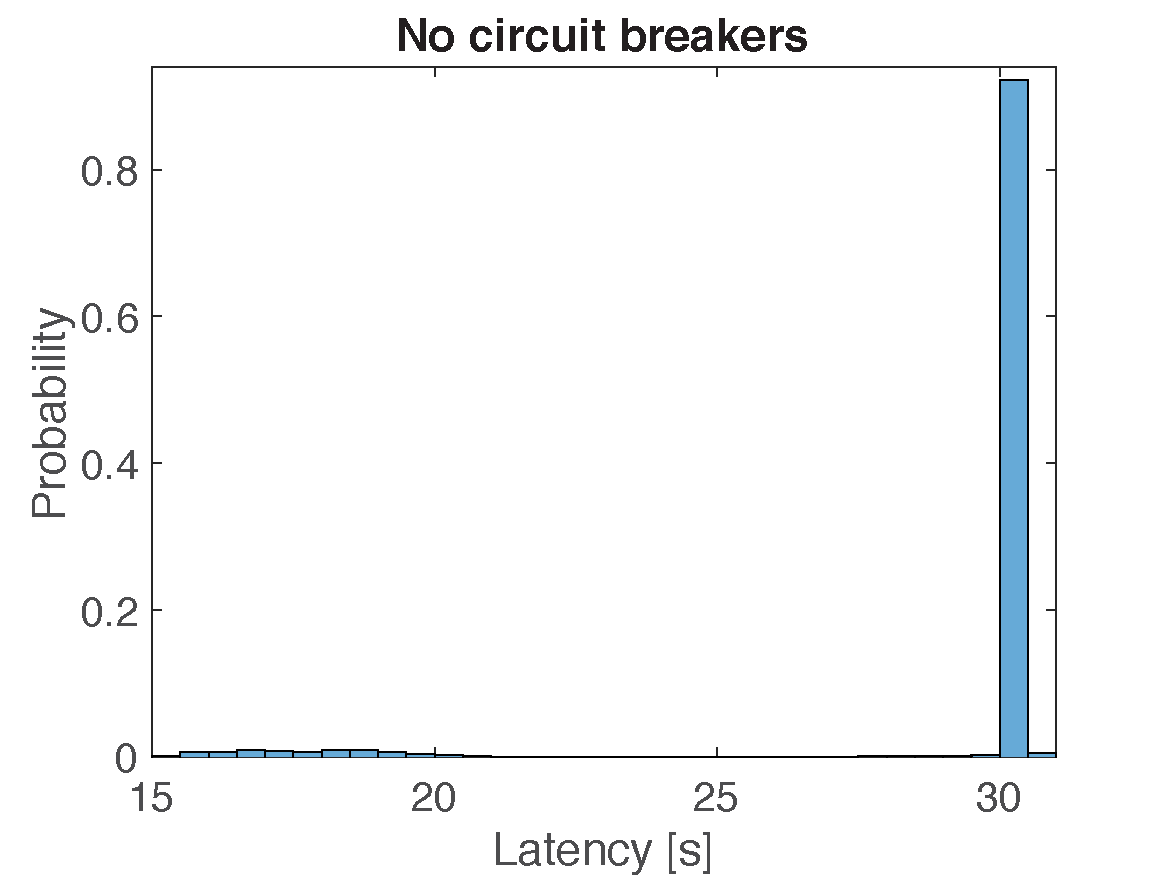
\includegraphics[width=7cm]{figures/nocb} }}%
          \qquad
    \subfloat[One circuit breaker]{{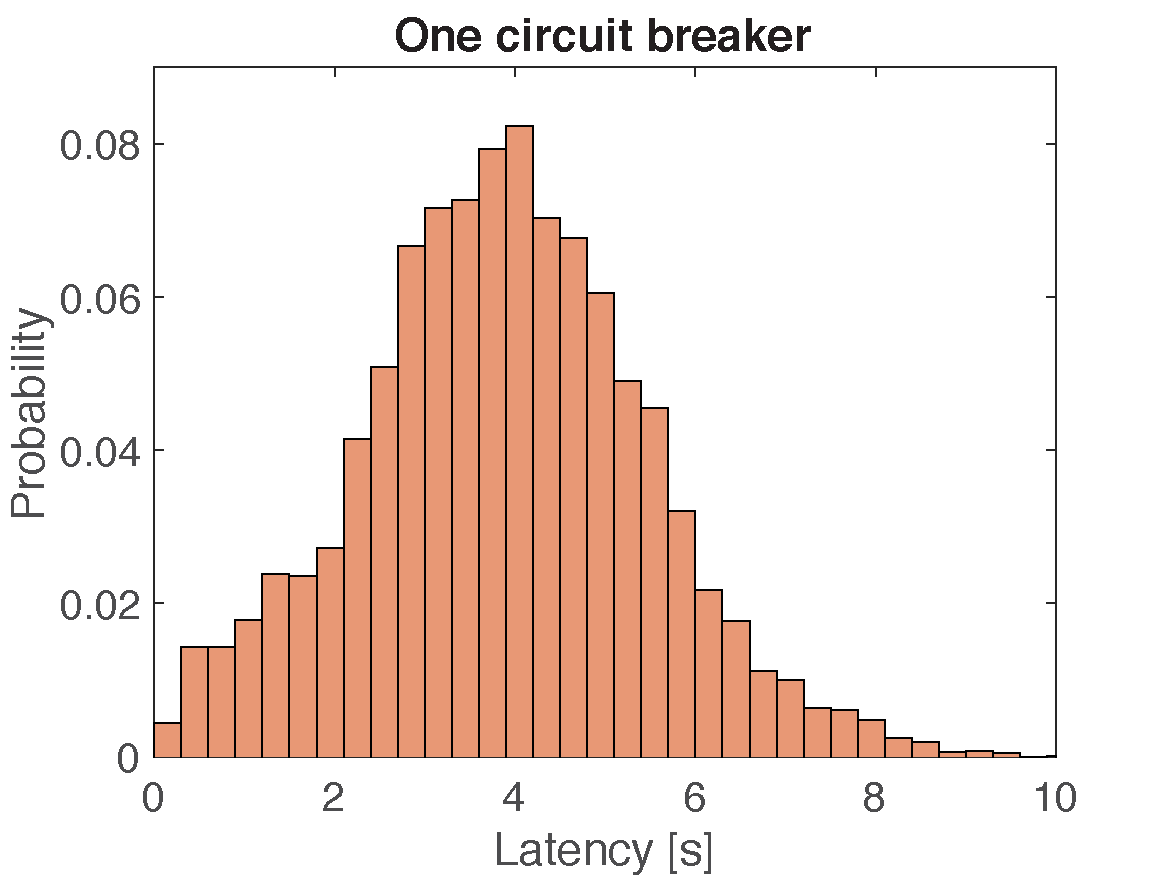
\includegraphics[width=7cm]{figures/onecb} }}%
          \qquad
    \subfloat[Two circuit breakers]{{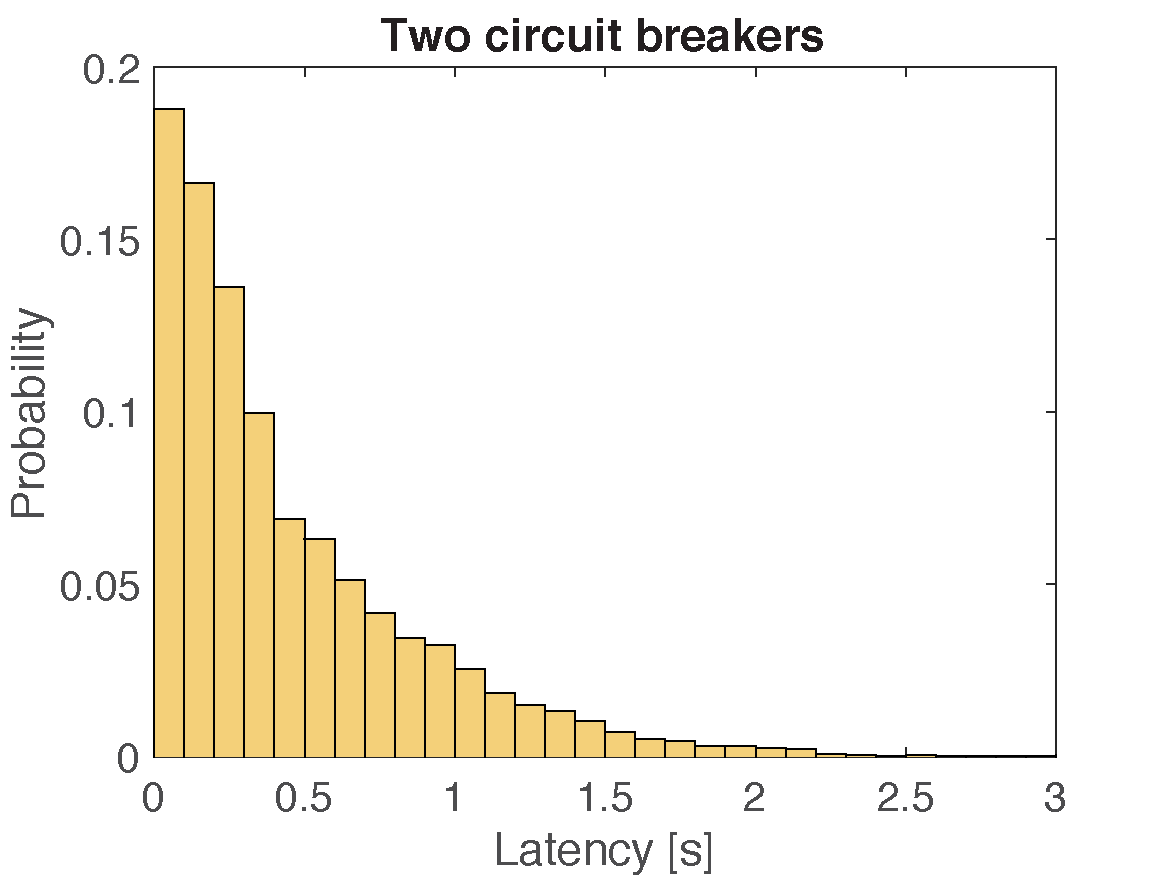
\includegraphics[width=7cm]{figures/twocb} }}%
    \caption{Effects of Circuit Breakers}%
    \label{fig:circuit_breakers}%
\end{figure}

\noindent
\textbf{Response Types} \\
The second part of the experiment is concerned with the degradation of the received content. This is an important factor in the experiment since the origin and success rate of the responses determine their usefulness. The distribution of the responses is sorted from best to worst (Table \ref{circuit_breaker_table}), and it is seen that responses from Service 2 only were obtained without using circuit breakers. This makes sense since circuit breakers, in the other scenarios, have a timeout at 1 second and Service 2 sleeps for 15 seconds for each request. The 7.2778\% succeeding answers in the first scenario came at the expense of 92,7222\% timeouts.

\noindent
Applying a circuit breaker in Service 1 led to almost nothing but responses from Service 1's fallback method, but a few server errors with HTTP status code 500 were also received. The fallback method is invoked when the circuit breaker's state is open. The 0,0111\% server errors correspond to 1 of 9000 responses.\\

\noindent
Applying two circuit breakers, the distribution of response origins is mainly split between Service 0 and Service 1's fallback methods.

\renewcommand*{\arraystretch}{1.6}
\setlength\LTleft{0pt}
\setlength\LTright{0pt}
\begin{longtable}{@{\extracolsep{\fill}}|p{3cm}|p{3.5cm}|p{3.5cm}|p{3.5cm}|} 
\hline
\rowcolor[HTML]{EFEFEF} & \textbf{No circuit breaker} & \textbf{One circuit breaker} & \textbf{Two circuit breakers} \\
\hline
\endfirsthead
\multicolumn{4}{c}%
{\tablename\ \thetable\ -- \textit{Continued from previous page}} \\
\hline
\rowcolor[HTML]{EFEFEF} & \textbf{No circuit breaker} & \textbf{One circuit breaker} & \textbf{Two circuit breakers} \\
\hline
\endhead
\hline \multicolumn{4}{r}{\textit{Continued on next page}} \\
\caption{Distribution of response types}
\endfoot
\hline
\caption{Distribution of Response Types}
\label{circuit_breaker_table}
\endlastfoot

\textbf{Service 2} & 7.2778\% & 0\% & 0\% \\ \hline
\textbf{Service 1} & 0\% & 99.9889\% & 36.8111\% \\ \hline
\textbf{Service 0} & 0\% & 0\% & 62.7333\% \\ \hline
\textbf{Server error} & 0\% & 0.0111\% & 0.4556\% \\ \hline
\textbf{Timeout} & 92.7222\% & 0\% & 0\% \\ \hline

\end{longtable}

\noindent
In general, the scenario without circuit breakers failed 92.72\% of the time but was the only scenario getting a response from Service 2. The scenario with a single circuit breaker reduced the response time significantly, and the degradation of the response was better than the last scenario. The scenario with two circuit breakers was even faster and shifted the degradation of the responses to Service 0's fallback method in most cases.

\subsection*{Discussion of Experiment: Integration Points in a Synchronous Architecture}
Consistency in the responses is traded for availability, as seen from the results (Table \ref{circuit_breaker_table}). The scenario without circuit breakers was the only experiment obtaining answers from the desired service (Service 2), but 92.7\% of the responses timed out, which leads to an availability percent of 7.3\%. Adding a circuit breaker in Service 1 shifts the availability to 99.99\% with a timeout at 30 seconds. Consistency in the response is degraded since all the responses come from Service 1 instead of Service 2. Adding another circuit breaker in Service 0 results in 99.5\% availability. The degradation of the responses contained 36.8\% responses from Service 1 and 62.7\% responses from Service 0.  \\

\noindent
The shift in latency (Figure~\ref{fig:circuit_breakers} (a)) clearly shows an improvement in latency by using a circuit breaker. A way of obtaining resilience is, thereby, by protecting against slow responses from integration points. \\



\noindent
An important aspect of the experiment is to design the test protocol to start from the same state for each iteration. The services had a startup delay that caused the first request to time out. Therefore, it was necessary to ensure that the services were ready before each test.
Two requests to Service 0 were made before starting the test to make sure that all three services had started. Furthermore, executing two tests without resetting the state led to different results. The reason for this were probably Service 2's blocked threads and state in the circuit breakers. Therefore, the services were removed and created between each testrun.

\newpage
%%% Experiment 1.2 Infrastructure
\section{Infrastructure Level Experiments}\label{sec:exp_replication}
The previous section focused on the effects of application level patterns to achieve a higher degree of resilience. This section will instead look into designing experiments to verify the different initiatives possible at the infrastructure level. Fault tolerance and the ability to detect failures are among the most notable features to ensure a higher degree of resilience at the infrastructure level, as described in Chapter~\ref{chap_fundamentals_resilient_cloud}.

\subsection*{Design of Experiment: Effects of Replication}
Fault tolerance is a key feature in Kubernetes. The goal of this experiment is to investigate the effects of replication to determine the how number of replicas affects the latency under varying traffic loads.  \\ 

\noindent The test setup consists of a simple application written in Java with the Spring Boot framework. The application is packaged into a Docker container and deployed into Kubernetes. The application is returning a string when it receives a HTTP request at '/'. The experiment performs ramp up of requests, which refers to continuing to apply an increasing amount of load, to stress the system. 10.000 requests are performed at each step with a step size at 100 requests/second until the system experience a drastic increase in latency. Calculating the duration of each step is done using the following formula: \\

\[ duration_{step}
  = \dfrac{10.000 + (rate_{current}-1)}{rate_{current}}
\] \\

\noindent
This experiment is performed with three scenarios: replicas=1, replicas=5, and replicas=10. Each scenario runs three times to eliminate randomness and the worst outliers. The average response time of the three runs of each step is applied. All load is generated by a MacBook Pro through a cabled network directly at the service endpoint '/'. \\

\noindent
The expected result is that replicating the application will move the boundary for failure. \\

\noindent\textbf{Test Protocol}\\
Every test shall be run with a 'clean' environment. The test protocol of this experiment is as follows:

\vspace{-3mm}
\begin{enumerate}
  \setlength\itemsep{0.05em}
  \item Run the application in Kubernetes (start the pod)
  \item Expose the application in Kubernetes (add a service)
  \item Scale the deployment to the desired number of replicas
  \item Start the test script \footnote{Attachment 6}
\end{enumerate}

\noindent
Steps 1-4 shall be run in total of three times.\\


\noindent\textbf{Metrics}\\
The main metric in this experiment is \textit{latency} and \textit{the number of replicas}. Especially the point at which the latency will have a drastic increase is the point of interest. \\

\noindent\textbf{Data Basis}\\
Three iterations of each scenario are run to reduce the impact of random factors. The result of each step for each scenario is an average of 30,000 measurements.

\subsection*{Results of Experiment: Effects of Replication}

The results of running the described test protocol verify the boundary for failure is moved when increasing the number of replicas. Figure~\ref{fig:rep_effect} shows the result of the experiment. Each scenario is depicted as a fitted line to each step's average of the latencies for each iteration. 

\begin{figure}[H]
\centering
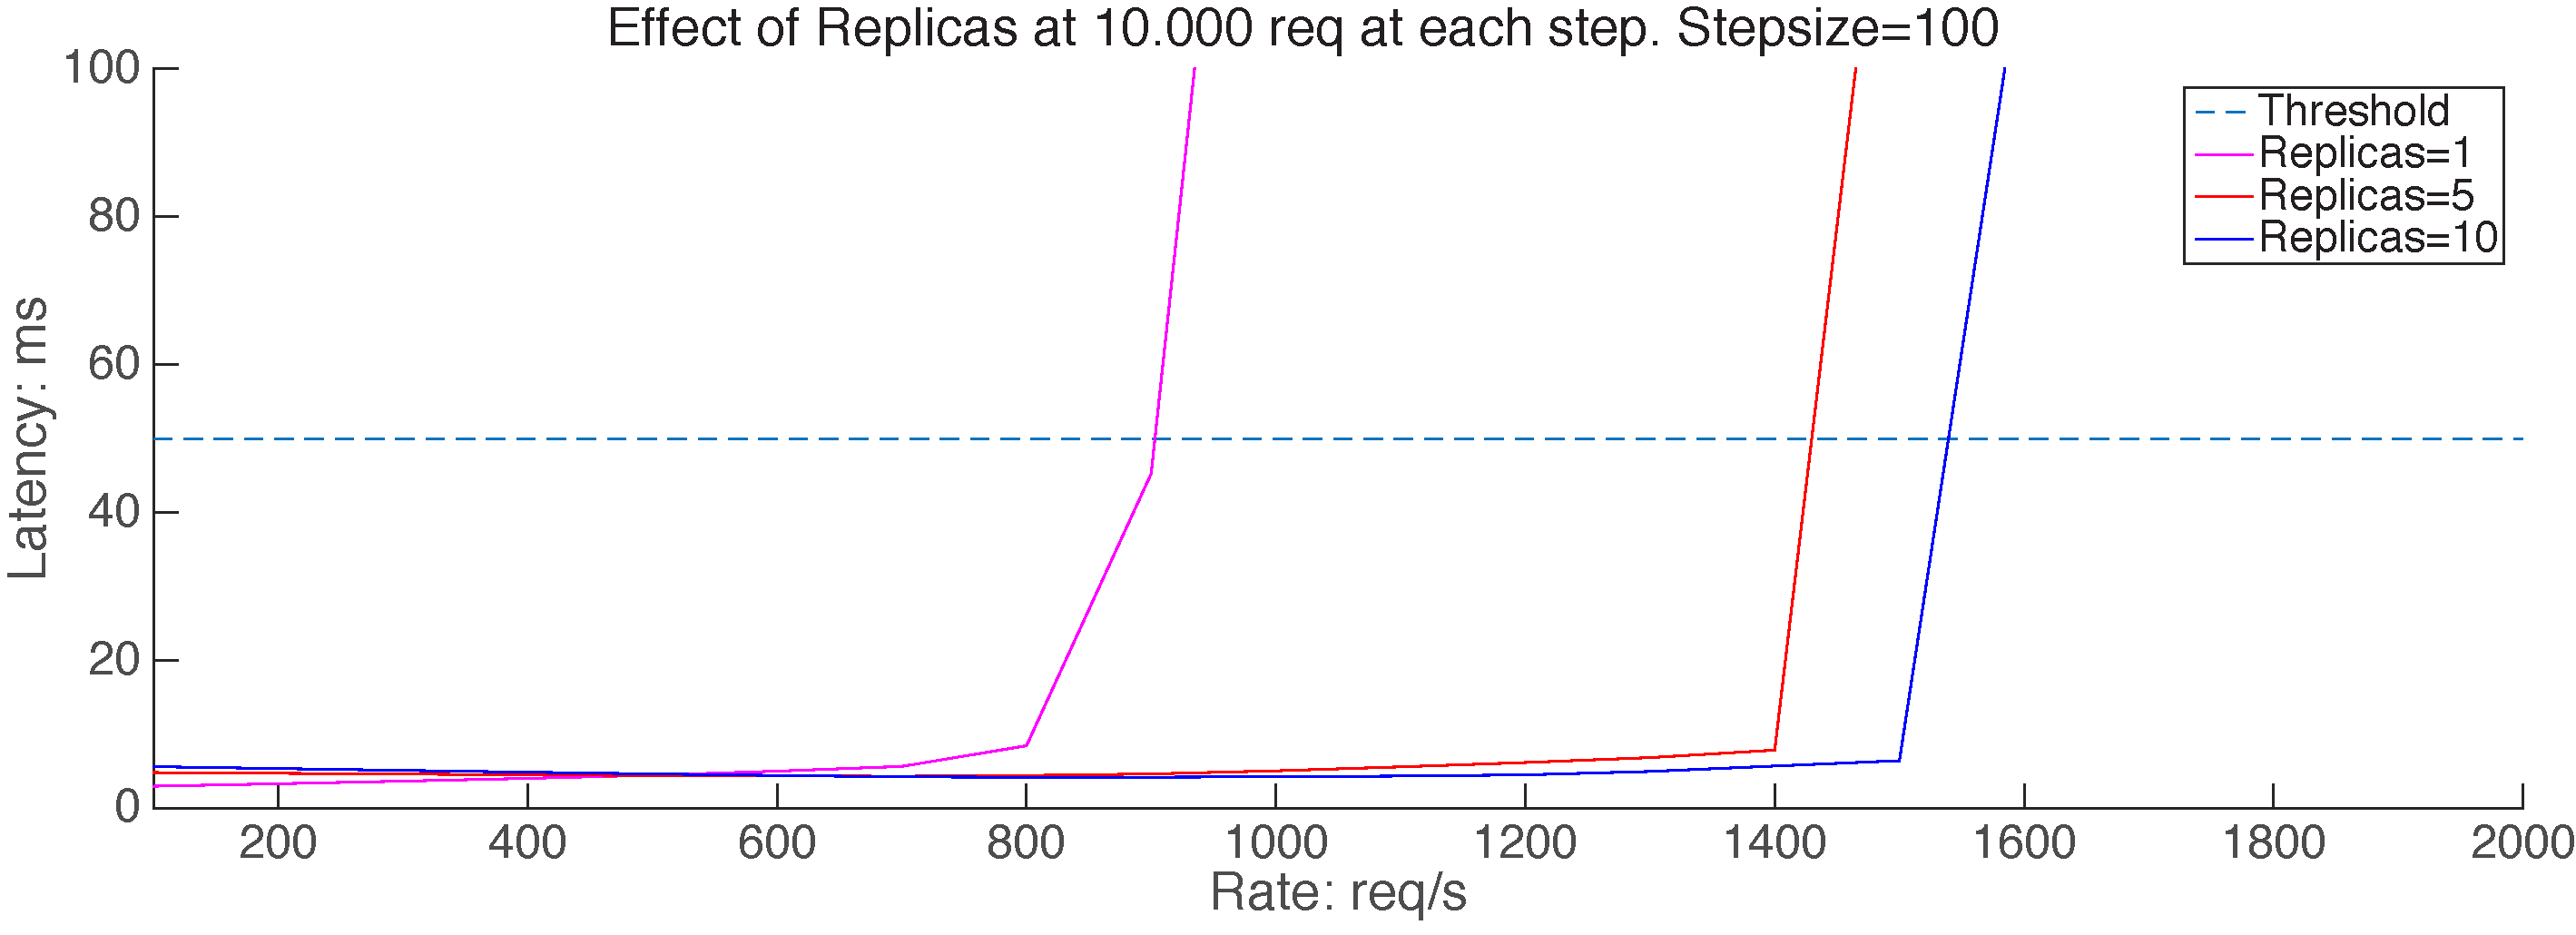
\includegraphics[width=\textwidth]{figures/effect_of_replicas_at_10000req_each_step}
\caption{Effects of Replicas at 10.000 Req. each Step}
\label{fig:rep_effect}
\end{figure}

\noindent Figure~\ref{fig:rep_effect} shows the effect of using an infrastructure with replication. The threshold applied to Figure~\ref{fig:rep_effect} is a reference point, determining an unsatisfiable latency. At some point, a drastic increase begins, and the server becomes unresponsive shortly hereafter. The iteration of the scenario is stopped when timeouts pile up. The results can be summarized to:
\begin{table}[]
\centering

\begin{tabular}{|l|l|}
\hline
\rowcolor[HTML]{EFEFEF} 
                     & \textbf{Breaking point}   \\ \hline
\textbf{Replicas=1}  & $\sim$900 request/second  \\ \hline
\textbf{Replicas=5}  & $\sim$1400 request/second \\ \hline
\textbf{Replicas=10} & $\sim$1500 request/second \\ \hline
\end{tabular}
\caption{Effects of Replicas Summarized}
\label{table:effects_replicas}
\end{table}

\noindent Increasing the number of replicas from 1 to 5 shifts the amount of concurrent request that the system can handle from 900 request/second to 1400 request/second, which is an increase of 55.6\% in the amount of load that the application can handle. The improvement of using 10 replicas instead of 5 replicas is significantly lower, and it only provides an increase in requests/second of 7\% compared to 5 replicas.
 
 
\subsection*{Discussion of Experiment: Effects of Replication}
From the experiment, it is seen that the number of replicas has a correlation with the throughput. The robustness of a system is concerned with how well it withstands stress, and from the results, it is seen that adding more replicas pushes the limit of requests/second it can handle (Figure~\ref{fig:rep_effect}). \\

\noindent
The improvement in performance from 1 to 5 replicas is significant, but from 5 to 10 replicas the improvement is less significant. A reason for this might be that the cluster consists of four Raspberry Pis, and the resources are more or less utilized.

\noindent
During the tests, the system was pushed beyond its boundaries which resulted in peculiar behavoir. Each iteration of each scenario required a shutdown of Kubernetes and a shutdown of the Raspberry Pis. This resulted in cumbersome waiting times.

%%% Experiment recovery time
\subsection*{Design of Experiment: Recovery Time}
Another key feature of Kubernetes as a platform is the ability to detect failures, e.g. a container failing or a node being removed from the cluster. The goal of this experiment is to look into this ability and try to determine the recovery time of an application, by only deploying one instance of the application. The second part of this experiment is to verify that by increasing the number of replicas the infrastructure will be able to handle a node failure with a minimum of lost requests. \\ 

\noindent The test setup consists of the same application used in the previous experiment. Since the goal of this experiment is to determine the effects of losing a node, the network cable of the node running the application will be pulled. The experiment will run with a total duration of 3 minutes (180 seconds) for each iteration, and the network cable is removed after 30 seconds. The experiment is run with replicas=1, replicas=2, and replicas=5 and with rate=100 request/second, and rate=200 request/second.\\

\noindent 
KubeCloud is configured with a timeout for unresponding nodes of 10 seconds (--node-grace-period) and a further timeout for the pods running on a unresponding node of 5 seconds (--pod-eviction-timeout). The expected result with one replica is that the application will be unresponsive for about 5 seconds (--pod-eviction-timeout) + 10 seconds (--node-grace-period) + 25 seconds (Spring Boot startup time on the Raspberry Pi) = 40 seconds. Whereas the expected result for running more than one replica will result in no period of unresponsiveness. \\

\noindent\textbf{Test Protocol}\\
Every iteration of a scenario has to be run with a 'clean' environment. The test protocol is as follows:
\begin{enumerate}
  \item Run the application in Kubernetes (start the pod)
  \item Expose the application in Kubernetes (add a service)
  \item Scale the deployment to the desired number of replicas
  \item Determine where the application (pod) has been started
  \item Start a stopwatch and test script at the same time
  \item After 30 seconds, remove the network cable of the node where the pod is running
\end{enumerate}
\noindent Steps 1-6 shall be run three times. If the application is scheduled on the master node, it is necessary to delete the pod and start it again to be rescheduled on a worker node. We only pull the plug of nodes with one application (pod) running. All load is generated by a MacBook Pro through a cabled network directly at the service endpoint '/'. \\

\noindent\textbf{Metrics}\\
The two main metrics in this experiment are \textit{the recovery time in seconds} and the \textit{success rate in percent}.\\

\noindent\textbf{Data Basis}\\
Three iteration of each scenario is run to reduce the impact of random factors.

\subsection*{Results of Experiment: Recovery Time}

The effect of applying replicas is clearly visible in regards to the recovery time and the ability of Kubernetes to detect a failure. Table~\ref{table:recovery_rates} summarizes the results of replication for the six scenarios run: replicas=1, replicas=2, and replicas=5 for rate=100 and rate=200. The results are averages of the three iterations of each scenario. 


\renewcommand*{\arraystretch}{1.8}
\setlength\LTleft{0pt}
\setlength\LTright{0pt}
\begin{longtable}{|p{5cm}|p{4cm}|p{4cm}|} 
\hline
\rowcolor[HTML]{EFEFEF} \textbf{Success rate} [\% (success/error)] & \textbf{rate=100} & \textbf{rate=200} \\
\hline
\endfirsthead
\multicolumn{3}{c}%
{\tablename\ \thetable\ -- \textit{Continued from previous page}} \\
\hline
\rowcolor[HTML]{EFEFEF} \textbf{Success rate} [\% (success/error)] & \textbf{rate=100} & \textbf{rate=200} \\
\hline
\endhead
\hline \multicolumn{3}{r}{\textit{Continued on next page}} \\
\caption{Comparison of Success Rates with Rate=100 and Rate=200}
\endfoot
\hline
\caption{Comparison of Success Rates with Rate=100 and Rate=200}
\label{table:recovery_rates}
\endlastfoot

\textbf{replicas=1} & 74.65\% (13,437/4,563) & 72.75\% (26,189/9,811) \\ \hline
\textbf{replicas=2} & 99.87\% (17,977/23) & 99.88\% (35,957/43)\\ \hline
\textbf{replicas=5} & 99.98\% (17,996/4) & 99,98\% (35,994/6)\\ \hline
\end{longtable}


\noindent The results show that the rate does not play a significant role. Furthermore, an improvement of approximately 25\% percentage points in the success rate between one replica and two replicas. The effect of running a single instance of the application is also clearly visible.  Figure~\ref{fig:recovery_rep1} shows a plot of one of the scenarios with rate=200 and one replica. The human factor involved in pulling the network cable resulted in slightly different timestamps for the unresponsiveness, therefore, a randomly selected scenario is shown to illustrate the differences. The plot in Figure~\ref{fig:recovery_rep1} shows a fitted line indicating successful requests (1) and failing requests (0) over time. 



\begin{figure}[H]
\centering
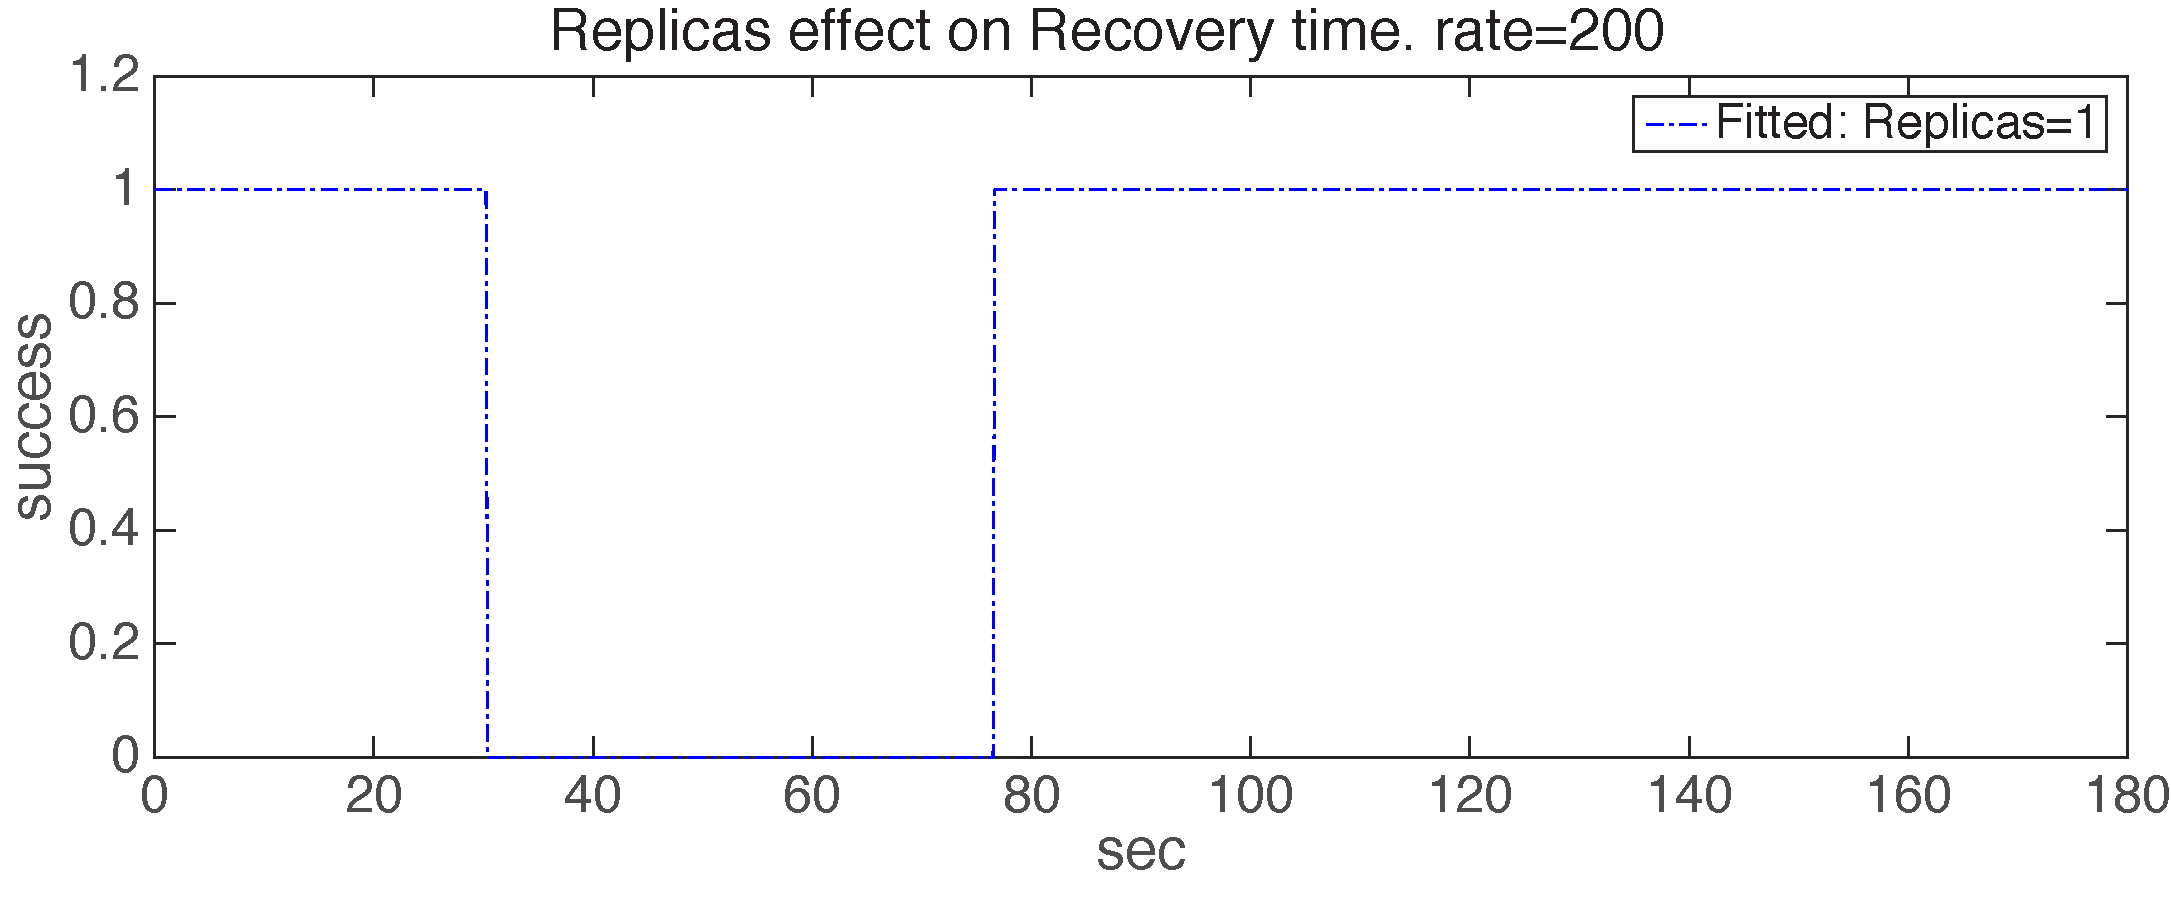
\includegraphics[width=12cm]{figures/recoverytime_rep1}
\caption{Replicas Effect on Recovery Time: Replicas=1, Rate=200}
\label{fig:recovery_rep1}
\end{figure}

\noindent 
It is clearly visible that the application is unresponsive, and that the client does not receive any responses for a total period of approximately 47 seconds. The 47 seconds is close to the expected recovery time of 40 seconds when running one replica.\\

\noindent Figure~\ref{fig:recovery_rep2} shows the effects of increasing the number of replications to a total of two. The effect of replication is, as stated in Table~\ref{table:recovery_rates}, clearly significant compared to only running a single instance as depicted in Figure~\ref{fig:recovery_rep2}.

\begin{figure}[H]
\centering
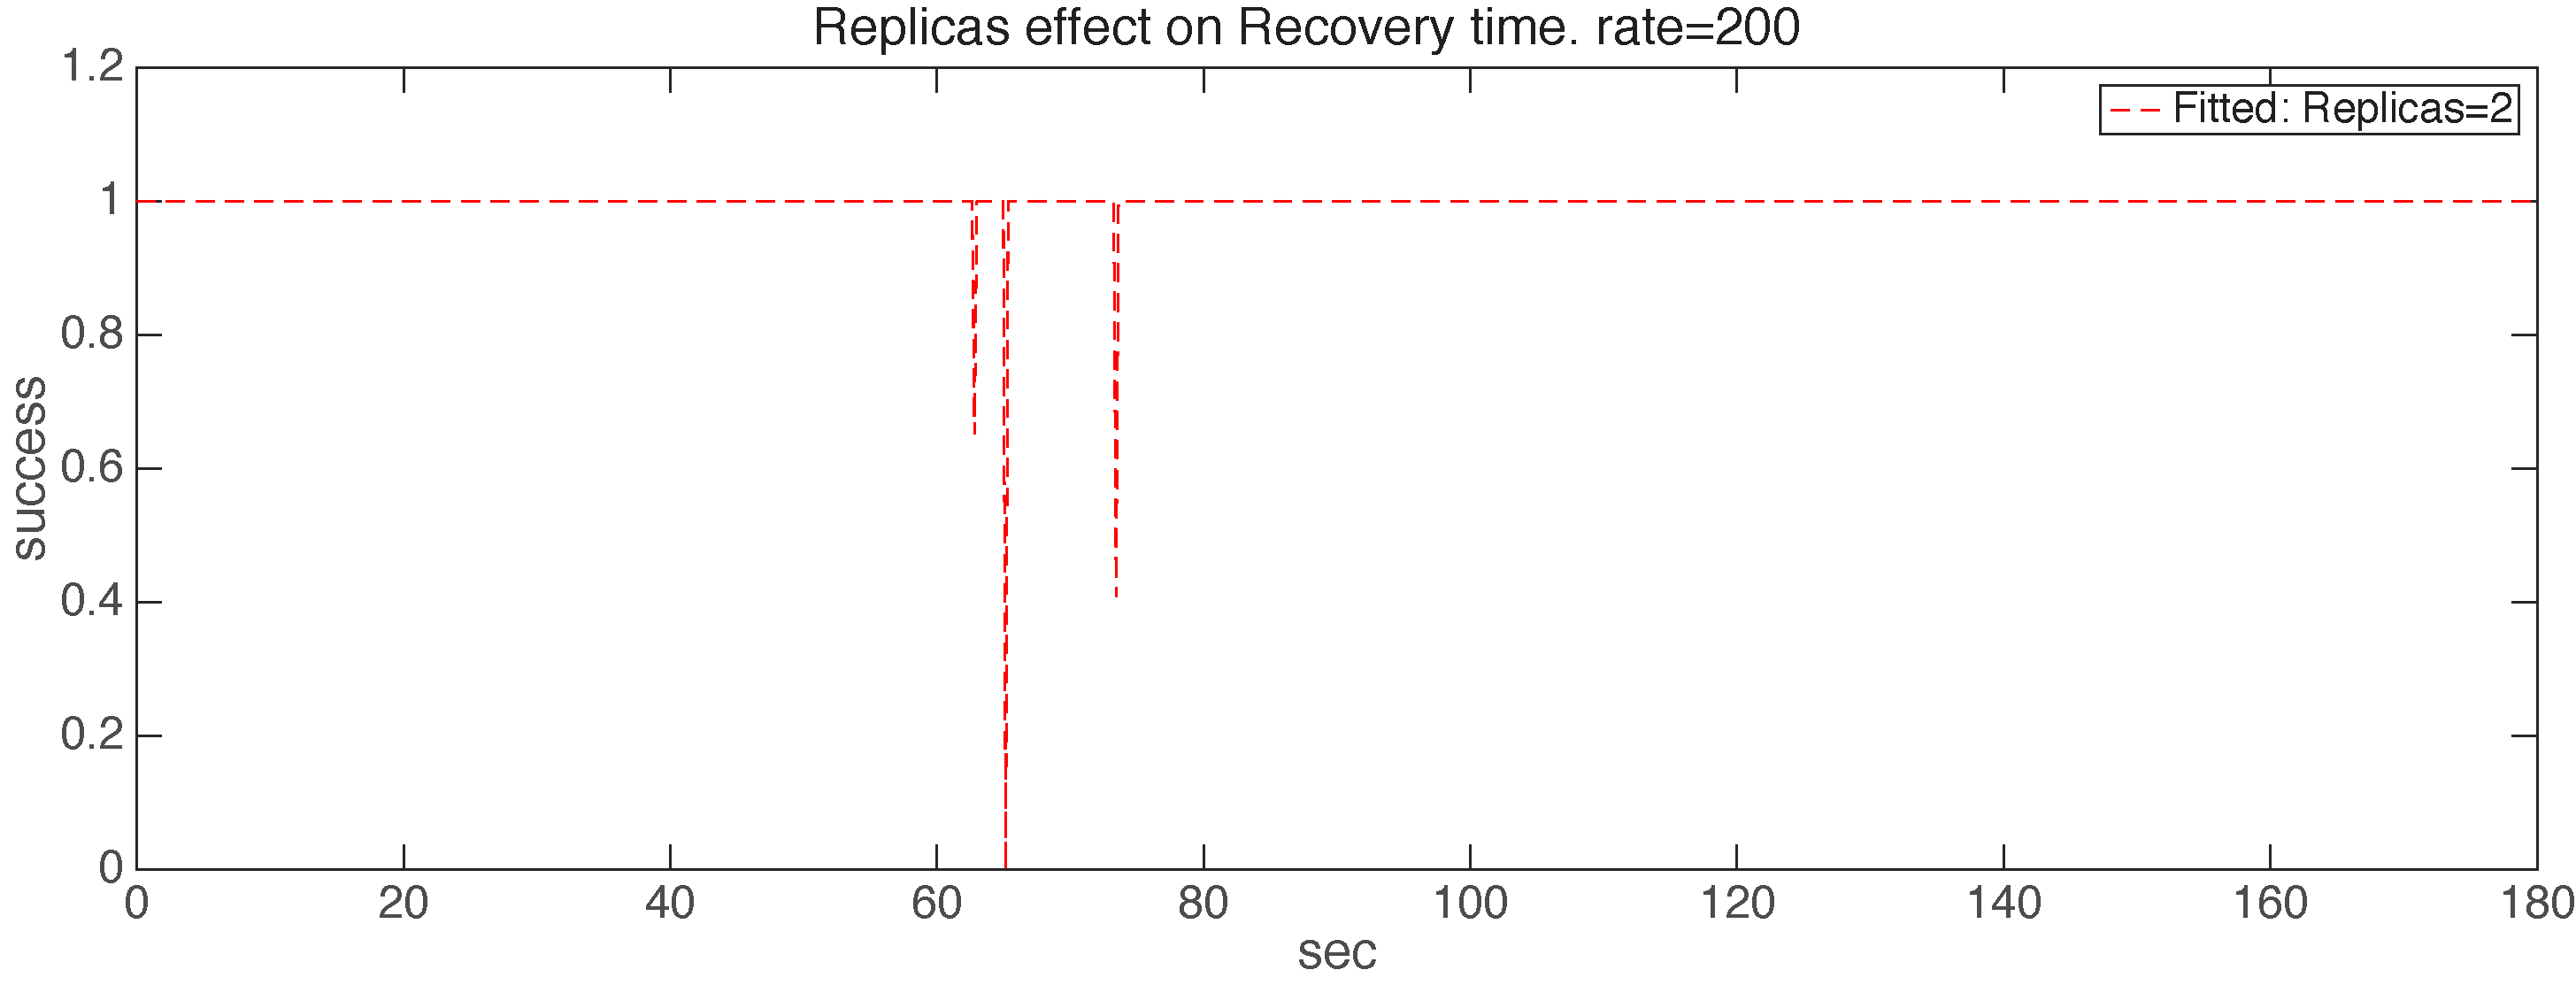
\includegraphics[width=12cm]{figures/recoverytime_rep2}
\caption{Replicas Effect on Recovery Time: Replicas=2, Rate=200}
\label{fig:recovery_rep2}
\end{figure}

\noindent
When running two instances the number of errors are on average reduced to 43 from 9,811 at rate=200. \\

\noindent
Lastly, Figure~\ref{fig:recovery_rep5} shows the effect of five replicas. The fitting of the line removes the on average six unsuccessful responses and the uptime is close to 100\%.
\begin{figure}[H]
\centering
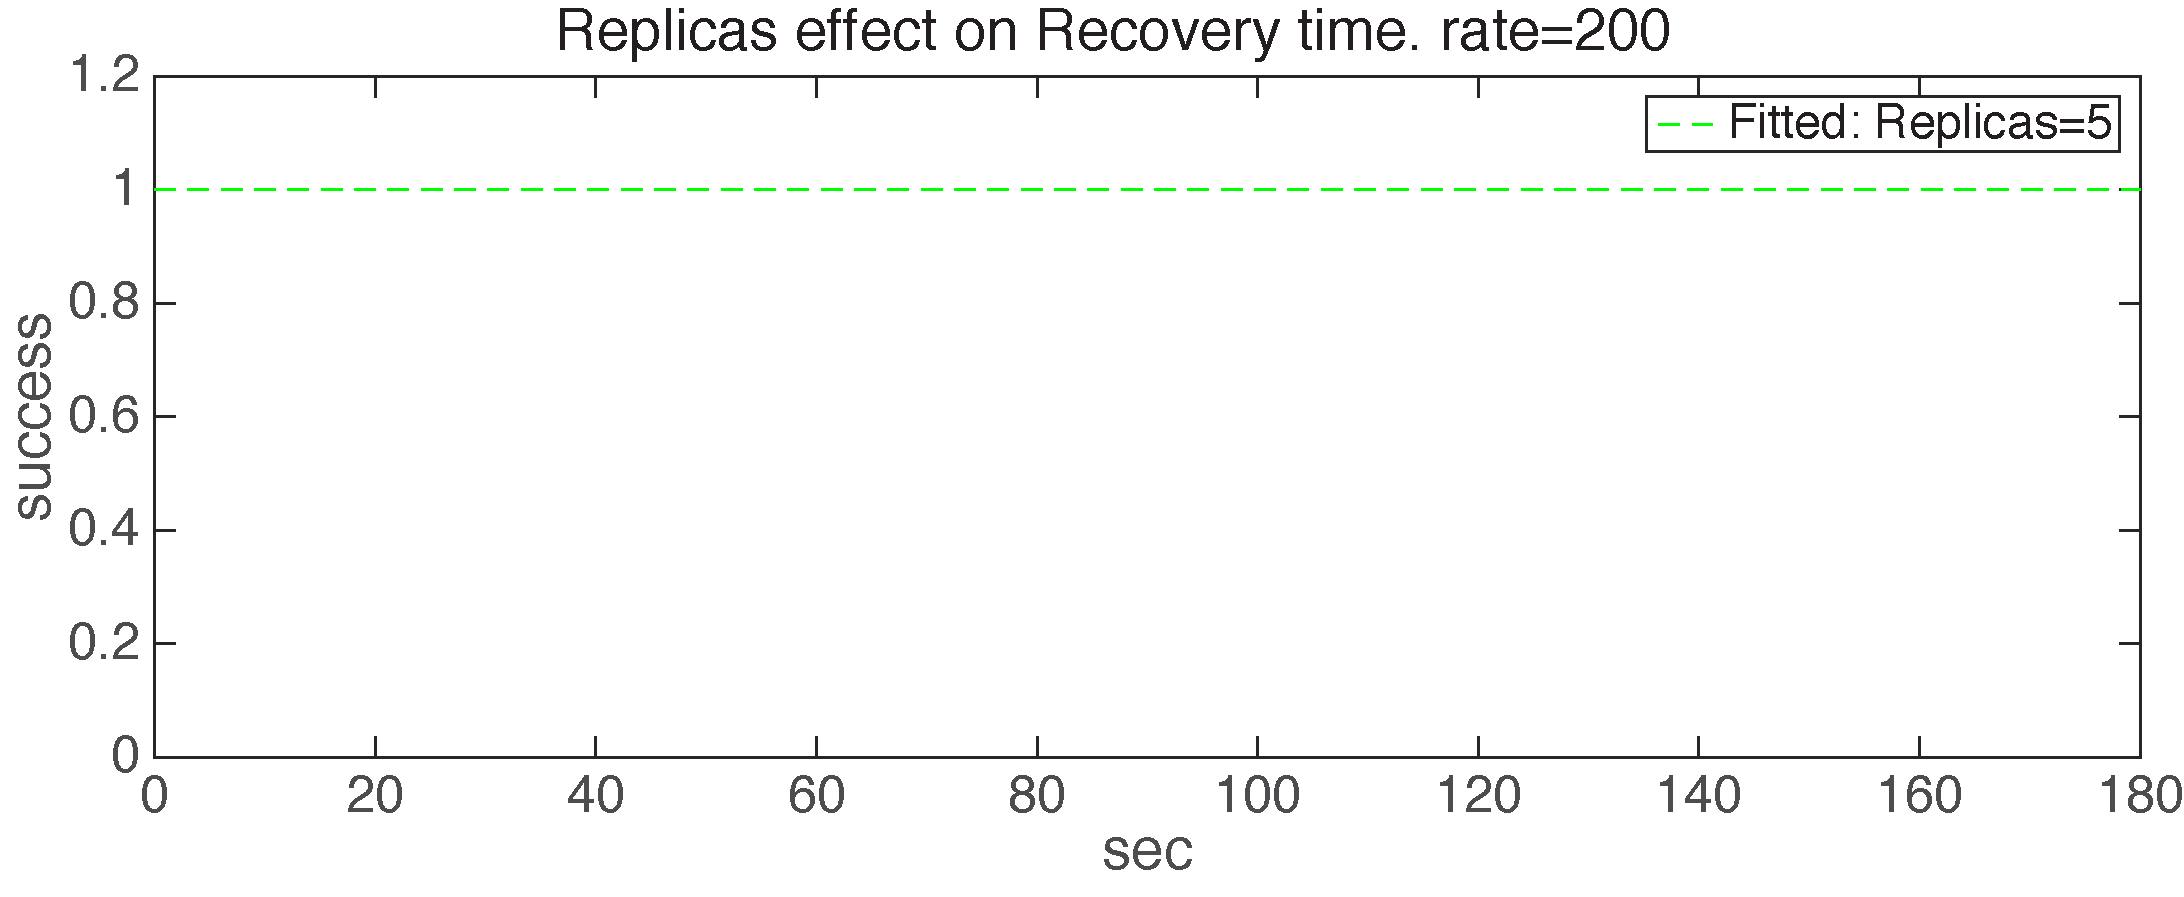
\includegraphics[width=12cm]{figures/recoverytime_rep5}
\caption{Replicas Effect on Recovery Time: Replicas=5, Rate=200}
\label{fig:recovery_rep5}
\end{figure}


\subsection*{Discussion of Experiment: Recovery Time}
The main conclusion is the importance of having more than one running replica at a time. The results show (Table~\ref{table:recovery_rates}) that an improvement from one to two replicas is very large, from around 73\% to around 99.9\%, while the further improvement is very small, but though present. It makes sense that an extra running instance can provide fault tolerance. \\

\noindent
Another desired attribute, in this case, is the rapidity of the infrastructure to identify and mitigate further errors. From the experiments, it is seen that Kubernetes quickly stopped traffic to the disconnected node. The configuration of Kubernetes' timeouts (--pod-eviction-timeout and --node-grace-period) especially played a role in the first scenario in which no other node could respond instead. \\


%\section{Design of experiments}
%%!TEX root = ../../master.tex




%\subsubsection*{Experiment 2.1.2 - Latency injection} 
%
%\textbf{Test protocol}
%\textbf{Metrics}
%Latency, success rate, content
%\textbf{Data basis}


%
%
%\section{Results}
%%!TEX root = ../../master.tex




%\subsubsection*{Experiment 2.1.2 - Latency injection} 




%
%\section{Discussion}
%\label{sec:experiment2_discussion}
%%!TEX root = ../../master.tex




